\section{ANALISIS E INTERPRETACION DE RESULTADOS} 
-Al compilar el proyecto de prueba, las pruebas aparecen en el Explorador de pruebas. Si el Explorador de pruebas no está visible, elija Prueba en el menú de Visual Studio, elija Ventanas y, después, Explorador de pruebas.
-Se puede elegir Ejecutar todas para ejecutar todas las pruebas o bien Ejecutar para elegir un subconjunto de pruebas que se desea ejecutar. Después de ejecutar un conjunto de pruebas, aparecerá un resumen de la serie de pruebas en la parte inferior de la ventana Explorador de pruebas. Seleccione una prueba para ver los detalles de esa prueba en el panel inferior. 
\begin{enumerate}[1.]
	\item Pruebas Unitarias
	\begin{enumerate}[a)]
	\item Paso 1: Pruebas unitarias: haremos pruebas unitarias para los métodos deposito, retiro.\\
		-  Agregaremos un test de pruebas unitarias
		\begin{figure}[H]
		\begin{center}
		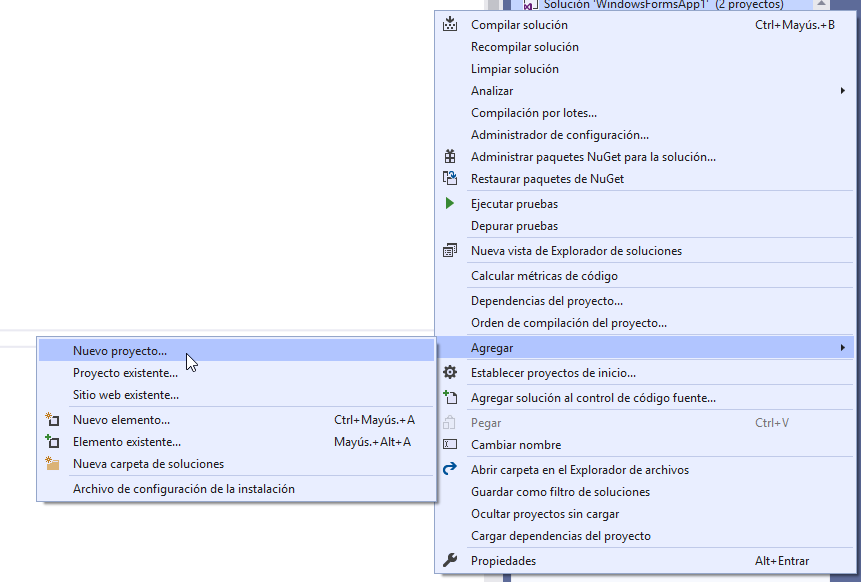
\includegraphics[width=8cm]{./Imagenes/imp1}
		\end{center}
		\end{figure}
	\item Paso 2: Seguidamente el nuevo y tipo de proyecto.
		\begin{figure}[H]
		\begin{center}
		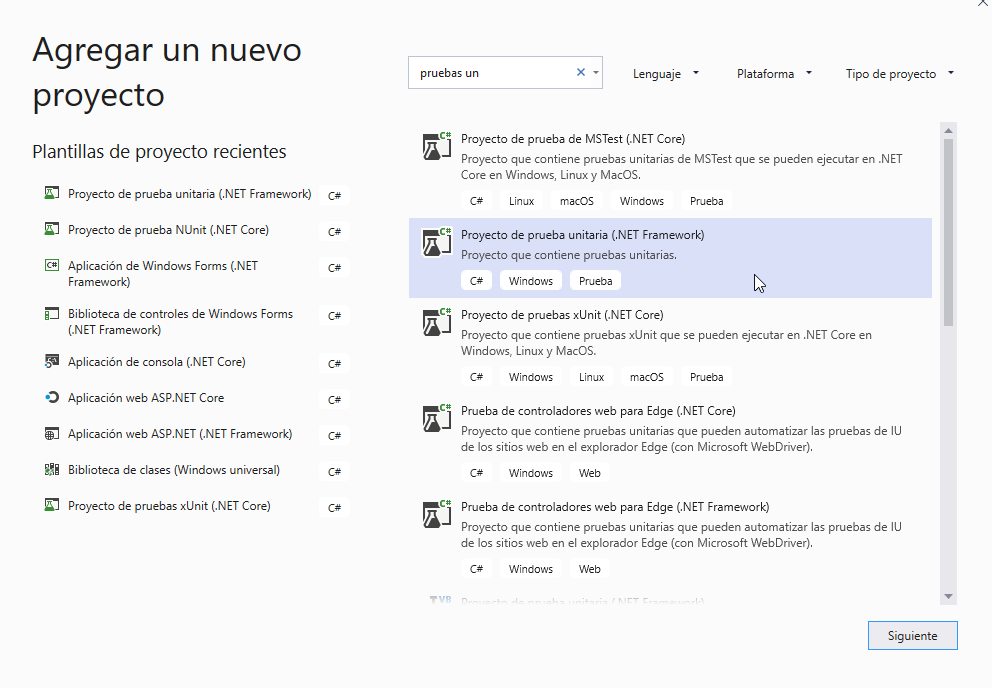
\includegraphics[width=6cm]{./Imagenes/imp2}
		\end{center}
		\end{figure}
	\item Paso 3: Luego referenciaremos el proyecto principal
		\begin{figure}[H]
		\begin{center}
		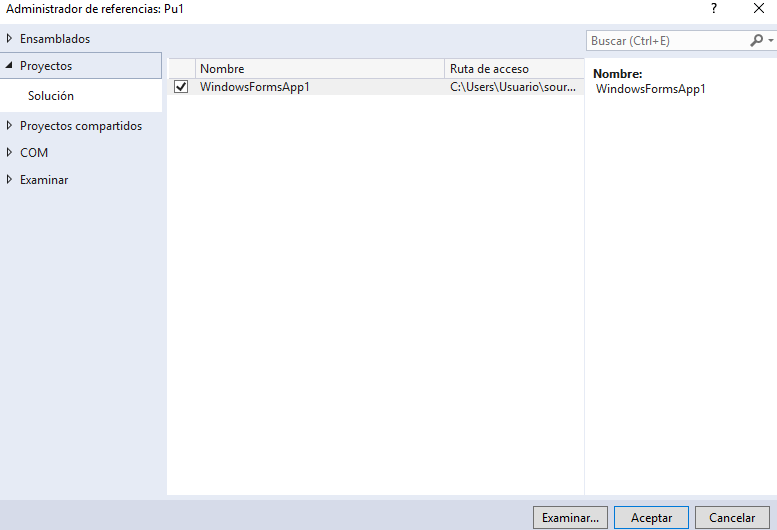
\includegraphics[width=6cm]{./Imagenes/imp3}
		\end{center}
		\end{figure}
	\item Paso 4: Luego probaremos los métodos :
		\begin{figure}[H]
		\begin{center}
		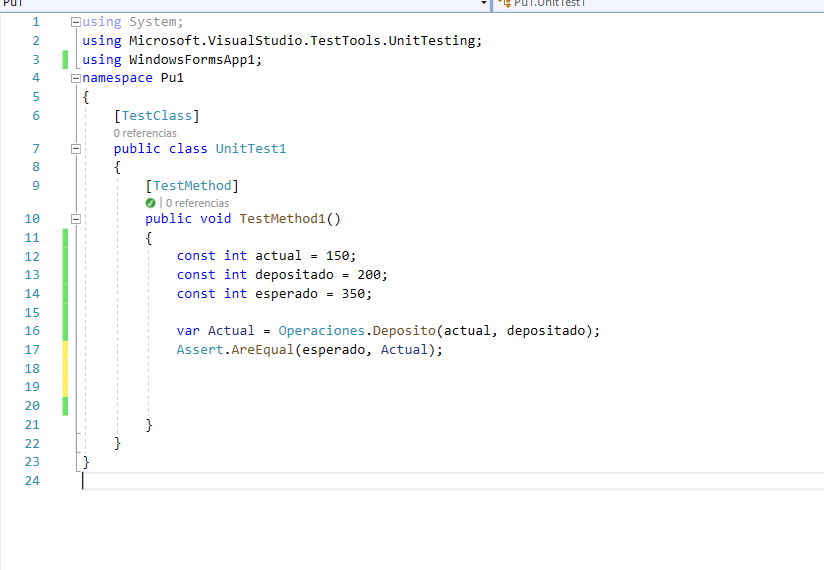
\includegraphics[width=7cm]{./Imagenes/imp4}
		\end{center}
		\end{figure}
	\item Paso 5: Esperamos mientras carga la pruba que se va desarrollar
		\begin{figure}[H]
		\begin{center}
		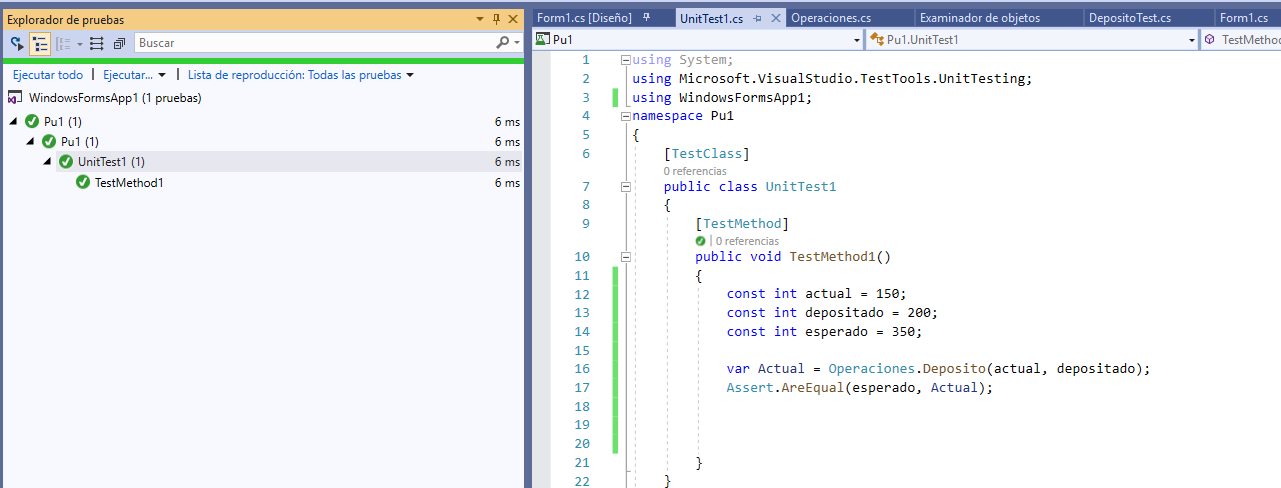
\includegraphics[width=6cm]{./Imagenes/imp5}
		\end{center}
		\end{figure}
	\item Paso 6: Retiros
		\begin{figure}[H]
		\begin{center}
		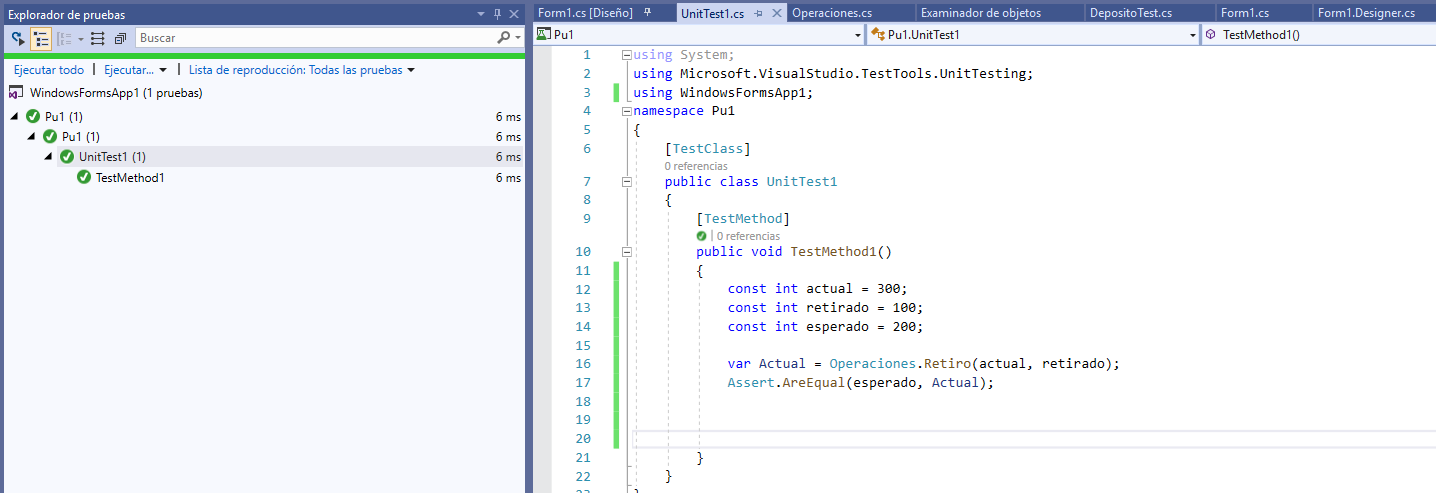
\includegraphics[width=7cm]{./Imagenes/imp6}
		\end{center}
		\end{figure}
	\item Paso 7: Finalmente aplicamos el codigo que se ejecurtar
		\begin{figure}[H]
		\begin{center}
		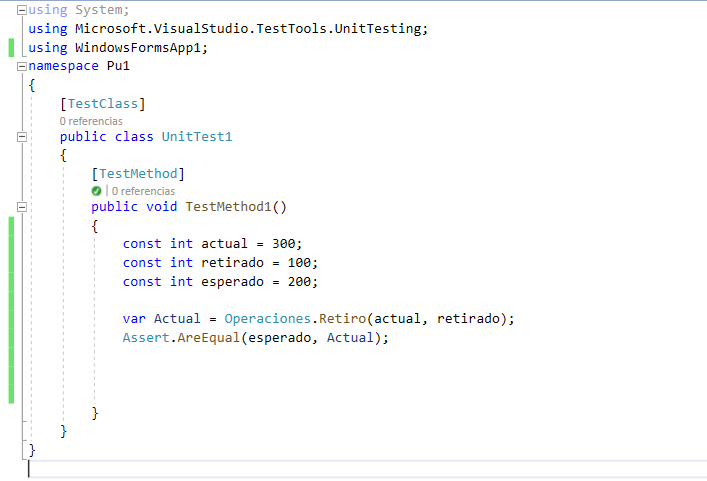
\includegraphics[width=7cm]{./Imagenes/imp7}
		\end{center}
		\end{figure}
	\end{enumerate}
\end{enumerate}